\chapter{Abordagem}
\label{sec:abordagem}

Este capítulo tem como principal objectivo descrever a metologia e ferramentas adoptadas e ainda apresentar o planeamento do projecto tal como os desvios relativamente ao mesmo. Por fim será apresentada uma analise dos riscos associados ao projecto que poderão tem um impacto negativo no plano de desenvolvimento. Este conjunto de passos foca-se em atingir um produto final bem estruturado e funcional, utilando boas práticas de desenvolvimento de software


\section{Metodologia}
\label{metodologia}

A metodologia de desenvolvimento do projecto adoptada foi uma metodologia fortemente baseada em SCRUM\cite{scrum}, que será descrita (i. e. os aspectos mais importantes) nesta secção. Esta é a metodologia utilizada pela 10.digital e tendo em conta que esta metodologia ágil se encaixa perfeitamente nas necessidades do projecto, estes foram os factos decisivos para a escolha da mesma. 





Equipa e tarefas de cada um.

\section{Ferramentas Utilizadas}
\label{ferramentas}


\section{Planeamento}
\label{planeamento}

\begin{figure}[ht!]
	\begin{center}
		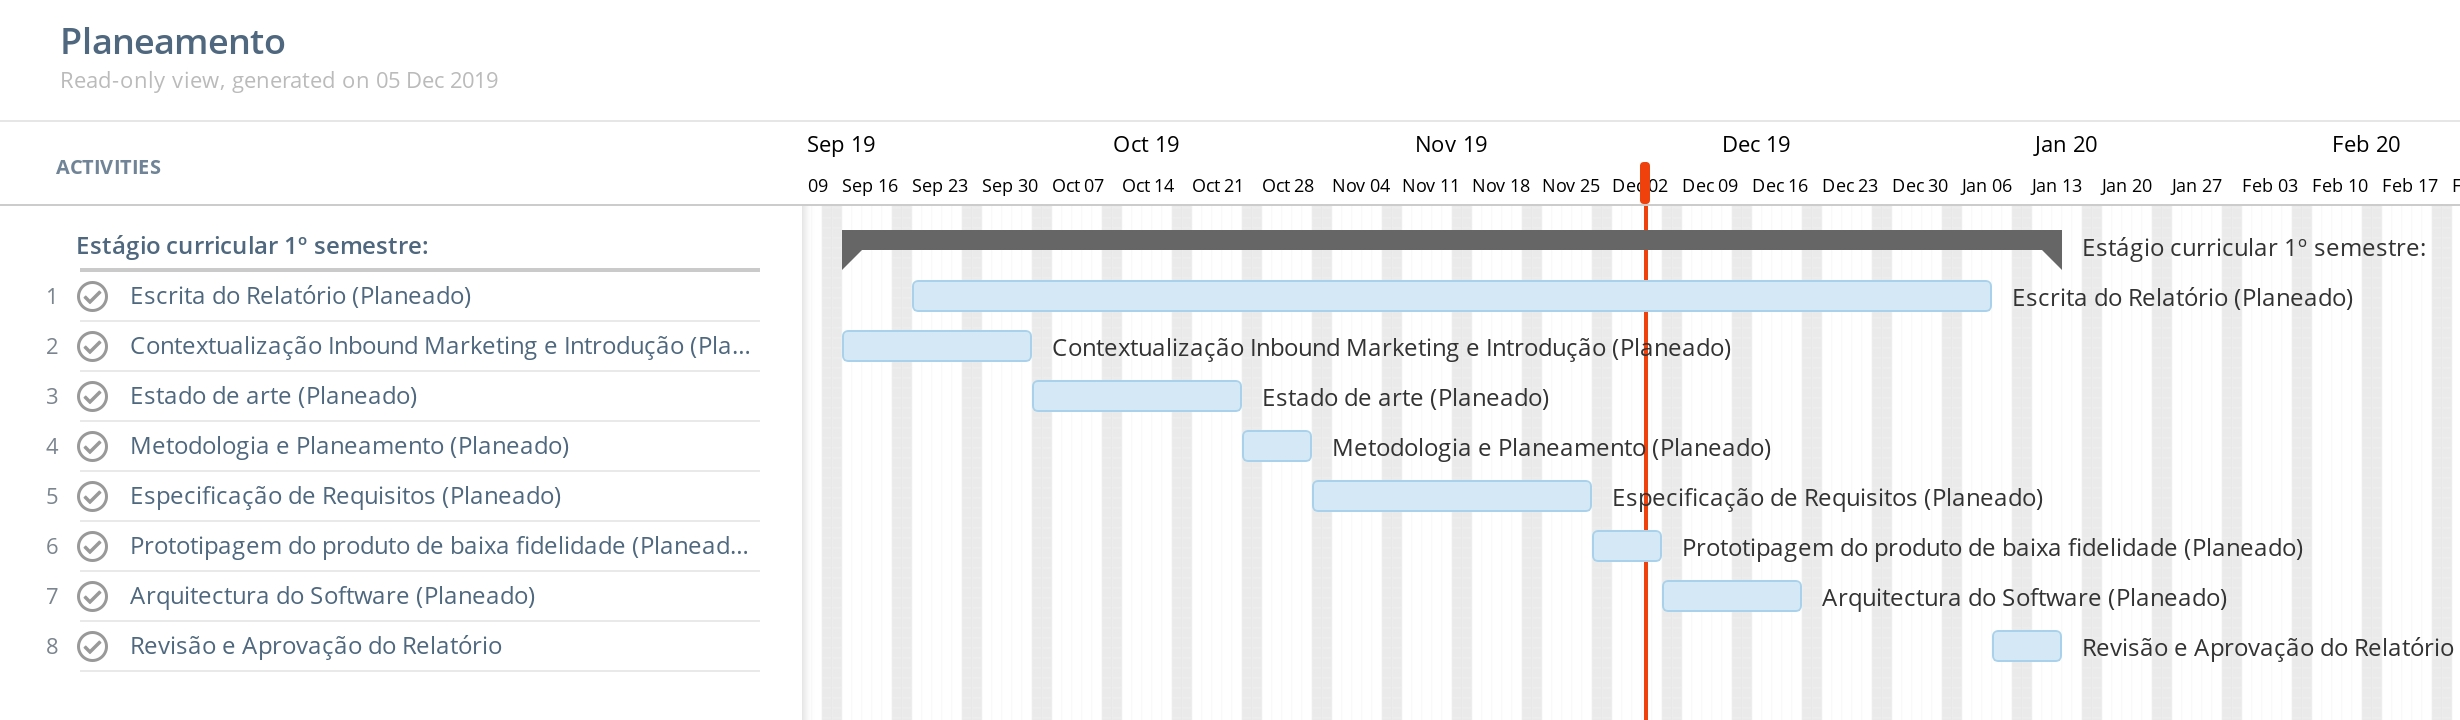
\includegraphics[width=1\textwidth]{img/gantt/semestre1.jpeg}
		\caption{Diagrama de Gantt - Planeamento do 1º semestre}
		\label{fig:gantt1}
	\end{center}
\end{figure}

\begin{figure}[ht!]
	\begin{center}
		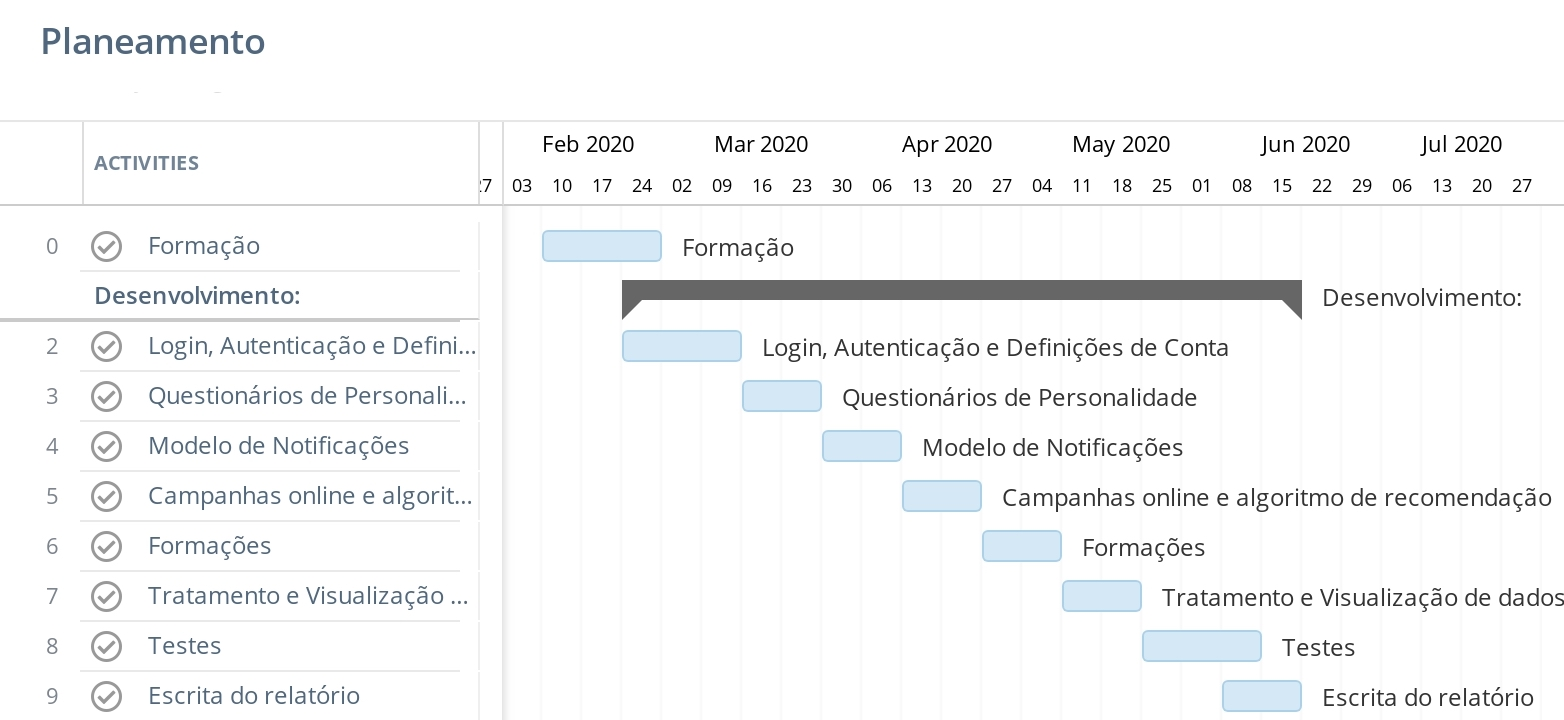
\includegraphics[width=1\textwidth]{img/gantt/semestre2.jpeg}
		\caption{Diagrama de Gantt - Planeamento do 2º semestre}
		\label{fig:gantt2}
	\end{center}
\end{figure}

\section{Analise se Riscos}
\label{analiseriscos}
%-------------------------------------------------------------------------------------------------
\blankpage
%-------------------------------------------------------------------------------------------------

\glsresetall



